\documentclass[conference]{IEEEtran}
\IEEEoverridecommandlockouts

% ==========================================
% PACKAGES
% ==========================================
\usepackage{cite}
\usepackage{amsmath,amssymb,amsfonts}
\usepackage{algorithmic}
\usepackage{algorithm}
\usepackage{graphicx}
\usepackage{textcomp}
\usepackage{xcolor}
\usepackage{booktabs}
\usepackage{multirow}
\usepackage{listings}
\usepackage{url}
\usepackage{float}

% --- TIKZ & PLOTS ---
\usepackage{tikz}
\usepackage{pgfplots}
\pgfplotsset{compat=1.17}
\usetikzlibrary{shapes.geometric, arrows, positioning, fit, calc, backgrounds, shadows}

% --- CODE STYLING ---
\lstset{
  basicstyle=\ttfamily\scriptsize,
  frame=single,
  breaklines=true,
  captionpos=b,
  numbers=left,
  numberstyle=\tiny\color{gray},
  keywordstyle=\color{blue},
  commentstyle=\color{green!50!black},
  stringstyle=\color{red},
  xleftmargin=2em,
  framexleftmargin=1.5em
}

\def\BibTeX{{\rm B\kern-.05em{\sc i\kern-.025em b}\kern-.08em
    T\kern-.1667em\lower.7ex\hbox{E}\kern-.125emX}}

\begin{document}

% ==========================================
% TITLE
% ==========================================
\title{Lifecycle Hardening of Immutable Edge Appliances under Power and Connectivity Instability}

% ==========================================
% AUTHOR
% ==========================================
\author{\IEEEauthorblockN{Dr. S. Suresh Kumar}
\IEEEauthorblockA{\textit{Department of Computer Science}\\
\textit{Swarnandhra College of Engineering \& Technology (Autonomous)}\\
Seetharampuram, Narsapur, Andhra Pradesh, India}
}

\maketitle

% ==========================================
% ABSTRACT
% ==========================================
\begin{abstract}
Edge-based academic deployments often operate as unattended embedded appliances installed in infrastructure-constrained environments. In such deployments, long-term reliability depends less on application accuracy and more on the stability of the underlying operating system and update lifecycle. In many institutional environments, these devices must tolerate unstable power conditions, intermittent connectivity, and limited opportunities for physical maintenance. Under such constraints, operating system configuration and lifecycle management frequently determine real-world viability more than application performance alone.

This study analyzes an immutable edge deployment architecture designed to improve corruption resistance and autonomous recovery under unstable power and connectivity conditions. We formalize an Appliance Invariance Model implemented through a read-only OverlayFS root structure that confines runtime mutations to volatile memory or versioned container layers. Additional safeguards include hardware watchdog integration tied to inference queue liveness and a Blue/Green Over-the-Air (OTA) update strategy with automated rollback logic.

Empirical validation on a controlled testbed subjected to repeated hard power interruptions and simulated update failures demonstrates stable reboot behavior and reliable automated recovery. The resulting system illustrates how disciplined operating-system immutability can improve reliability in distributed academic embedded appliances. Automated lifecycle control further strengthens system stability.
\end{abstract}

\begin{IEEEkeywords}
Embedded Systems, Reliability Engineering, OverlayFS, OTA Updates, Zero-Touch Provisioning, Fleet Management, Edge Appliances.
\end{IEEEkeywords}

% ==========================================
% I. INTRODUCTION
% ==========================================
\section{Introduction}

Deploying embedded systems as distributed edge appliances fundamentally changes the engineering priorities of infrastructure. Once installed in unattended environments, reliability becomes dominated by operating-system resilience, update safety, and autonomous recovery mechanisms rather than raw application performance. Although application accuracy and throughput remain important considerations, day-to-day reliability frequently depends on operating system stability and disciplined update management \cite{b1, b2, b3}.

Institutional deployments often expose edge appliances to unstable power conditions, intermittent networking, and restricted physical access. Power interruptions, wireless congestion, and restricted physical access are common. Under these conditions, conventional Linux deployments---particularly those relying on writable root filesystems---can gradually degrade or become unbootable over time \cite{b4, b12, b17}.

These constraints shift the engineering focus away from pure application optimization. Instead, emphasis moves toward deployment lifecycle and systems reliability engineering \cite{b6}. While prior research extensively covers application serving \cite{b7}, the operational lifecycle of the appliance ultimately dictates its real-world utility. An embedded application that achieves high accuracy in the laboratory provides little practical utility if its host OS fails to boot after a routine campus power outage.

This paper details an immutable, containerized OS architecture designed for Zero-Touch administration. By enforcing strict separation between the read-only host OS and the containerized inference logic, we ensure that the edge node can survive power loss, recover from software hangs, and securely update its models without human intervention. The system architecture and end-to-end data flow are assumed from the broader series; this study focuses exclusively on deployment lifecycle engineering and does not evaluate inference accuracy, storage endurance wear-leveling, or privacy enforcement.

% ==========================================
% II. FAILURE-STATE TAXONOMY & RELATED WORK
% ==========================================
\section{Failure-State Taxonomy and Related Work}

To analyze deployment reliability systematically, we categorize the primary failure classes encountered in unattended edge appliances:
\begin{itemize}
    \item \textbf{Power-Loss Corruption:} Unclean shutdowns mid-write causing OS unbootability (addressed via Appliance Invariance and OverlayFS).
    \item \textbf{Kernel Deadlock / Scheduler Exhaustion:} Total system freezes where software supervisors fail (addressed via Hardware Watchdog integration).
    \item \textbf{Application Crash:} Container-level segfaults or memory leaks (addressed via daemon process supervision and cgroup isolation).
    \item \textbf{Malicious Update Injection:} Poisoned firmware or rogue container deployment (addressed via TPM Secure Boot and pre-flight OTA validation).
    \item \textbf{Network Partition:} Multi-day loss of cloud connectivity (addressed via priority-aware buffering).
\end{itemize}

\subsection{MLOps for Edge Devices}
Although MLOps practices are well established in cloud infrastructure, their adaptation to distributed edge deployments remains comparatively underdeveloped. Sculley et al. \cite{b5} highlighted the ``hidden technical debt'' in ML systems, a problem that becomes significantly more challenging on distributed, constrained devices lacking standard data-center redundancies. Traditional edge deployment frameworks often lack the resilience required for environments with dirty power. Our work adapts cloud-native container orchestration concepts \cite{b8, b9, b10} to the embedded Linux context, relying heavily on kernel-level isolation and robust daemon supervision.

\subsection{Embedded Reliability and Filesystems}
Flash-based storage systems introduce additional reliability considerations when devices operate under unstable power conditions (particularly in embedded edge hardware) \cite{b12}. Journaling filesystems (like Ext4) provide metadata protection but cannot prevent corruption if the underlying flash translation layer is interrupted during an active block write \cite{b14}. The use of structural immutability to create read-only root structures has been explored to extend flash lifespans \cite{b13}, but its application to high-throughput, log-heavy edge appliances requires careful volatile memory management to prevent out-of-memory (OOM) cascading failures caused by RAM-disk exhaustion.

% ==========================================
% III. APPLIANCE INVARIANCE MODEL
% ==========================================
\section{Appliance Invariance Model}

The proposed deployment model treats the edge node as an immutable appliance instead of a conventional mutable Linux host. The system architecture and end-to-end data pipeline are defined by the broader architectural series; this work focuses on the lifecycle invariance properties of the deployment substrate. The deployment model intentionally avoids traditional package-manager operations such as remote apt-based upgrades executed through SSH. Instead, the host OS is treated primarily as a minimal read-only container runtime environment. All software dependencies, drivers, analytic logic, and neural network models are packaged into immutable Docker images \cite{b8}.

\subsection{Formal Invariant}
The architectural principle underlying this deployment strategy is formalized as the Appliance Invariance Model. Let $H$ represent the lower-layer persistent filesystem state, $C$ represent the containerized application state, and $V$ represent the volatile overlay state. The core system invariant is defined as:
\begin{equation}
\forall t,\; H_{persistent}(t) = H_0
\end{equation}

This invariant expresses the design principle that the persistent host operating system state should remain unchanged during routine operation. Runtime mutations are restricted either to volatile memory ($V$) or to versioned container layers ($C$) managed through controlled OTA transitions. In practice, this separation reduces the likelihood that repeated power interruptions accumulate filesystem inconsistencies over time.

\subsection{Immutability Layer Diagram}

\begin{figure}[htbp]
\centering
\resizebox{\columnwidth}{!}{
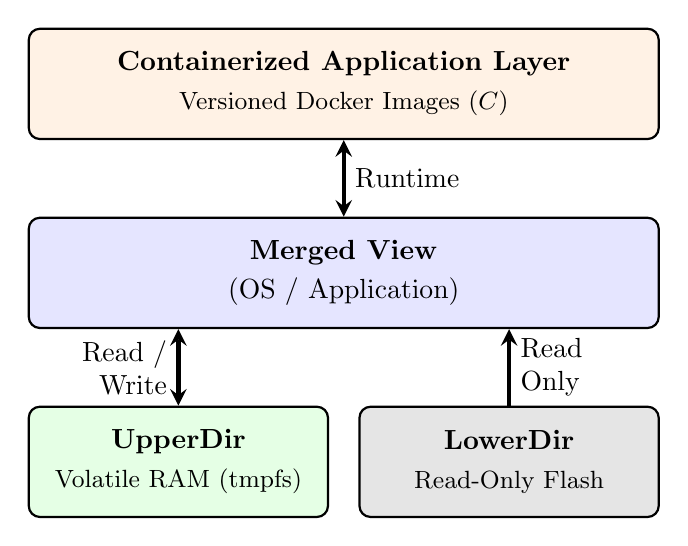
\begin{tikzpicture}[auto, thick, >=stealth,
    box/.style={draw, rectangle, rounded corners, align=center, minimum height=1.4cm}]
    
    \node [box, fill=blue!10, minimum width=8cm] (merged) at (0, 0) {\textbf{Merged View}\\[0.5ex] (OS / Application)};
    \node [box, fill=green!10, minimum width=3.8cm] (upper) at (-2.1, -2.4) {\textbf{UpperDir}\\[0.5ex] \small Volatile RAM (tmpfs)};
    \node [box, fill=gray!20, minimum width=3.8cm] (lower) at (2.1, -2.4) {\textbf{LowerDir}\\[0.5ex] \small Read-Only Flash};
    \node [box, fill=orange!10, minimum width=8cm] (container) at (0, 2.4) {\textbf{Containerized Application Layer}\\[0.5ex] \small Versioned Docker Images ($C$)};

    \draw [<->, ultra thick] (upper.north) -- node[left, align=right] {Read /\\Write} (upper.north |- merged.south);
    \draw [->, ultra thick] (lower.north) -- node[right, align=left] {Read\\Only} (lower.north |- merged.south);
    \draw [<->, ultra thick] (container.south) -- node[right] {Runtime} (merged.north);
\end{tikzpicture}
}
\caption{Appliance Invariance Architecture. The persistent lower layer ($H_0$) is never written to during normal operation. All runtime mutations are confined to the volatile UpperDir (RAM) or versioned container layers. Upon power loss, only the volatile layer is destroyed.}
\label{fig:overlay}
\end{figure}

This architectural decoupling ensures that the environment running the inference code is reproducible across fleet nodes provisioned from identical base images, standardizing deployment configurations and eliminating deployment friction.

% ==========================================
% IV. RELIABILITY ENGINEERING
% ==========================================
\section{Reliability Engineering}

System reliability emerges from the interaction of several complementary mechanisms implemented at the operating-system level. 

\subsection{Process Supervision}
The inference engine is operationalized as a system daemon using strict process-orchestration policies \cite{b16}. The unit configuration (Listing 1) defines strict restart policies. The \texttt{OOMScoreAdjust} directive explicitly protects the primary Docker daemon and SSH server from the Linux Out-Of-Memory (OOM) killer, shifting most memory exhaustion risk to the individual user-space containers which can be safely restarted without bringing down the host OS or losing network connectivity.

\begin{figure}[htbp]
\textbf{Listing 1: Supervisor Production Unit}
\begin{lstlisting}[language=bash]
[Unit]
Description=Edge Analytics Appliance
After=network.target docker.service
StartLimitIntervalSec=0

[Service]
Type=simple
Restart=always
RestartSec=3
User=root
# OOM Score: Protect Host Docker Daemon
OOMScoreAdjust=-1000
ExecStart=/usr/bin/docker-compose -f /opt/deploy.yml up
# Watchdog Integration
WatchdogSec=15s

[Install]
WantedBy=multi-user.target
\end{lstlisting}
\label{fig:systemd}
\end{figure}

\subsection{Hardware Watchdog Timer (WDT) Integration}

Software-level process supervision alone cannot recover from all classes of runtime failure. To address this, we enable the hardware Watchdog Timers (WDT) integrated into commodity ARM-based edge compute modules to provide hardware-level liveness enforcement for appliance survivability \cite{b15}. The watchdog ensures recovery under liveness failure; detailed runtime enforcement semantics and invariant verification are addressed in the architectural verification layer of the broader series.

\subsection{Read-Only Filesystem (OverlayFS) Mechanics}

Filesystem immutability is implemented using the OverlayFS union filesystem provided by the Linux kernel. To substantially reduce the likelihood of storage corruption during rolling blackouts, the root filesystem is mounted as read-only using OverlayFS. 

The physical storage acts as the immutable Lower Directory. A volatile \texttt{tmpfs} (RAM disk) is mounted as the Upper Directory. The operating system interacts with the Merged View. All system writes (logs, temp files, state changes) are seamlessly intercepted by the Linux kernel and written exclusively to the volatile RAM disk. 

Under this configuration, abrupt power removal destroys only the volatile UpperDir residing in RAM. Because persistent storage is mounted read-only during normal operation, boot-sector and base OS corruption events were not observed during evaluated power-cycle tests. While no filesystem configuration can eliminate all theoretical failure modes, this approach substantially reduces corruption exposure in environments with unstable power.

\subsection{RAM-Disk Exhaustion Mitigation}
To reduce the risk of RAM exhaustion, log output is aggressively bounded. System and container logs are capped, and cgroup-based memory ceilings are applied to inference containers. Because operational telemetry is streamed off-device when connectivity permits, deep local log retention is intentionally avoided.

% ==========================================
% V. OTA UPDATES & FLEET MANAGEMENT
% ==========================================
\section{OTA Updates \& Fleet Management}

Maintaining a distributed fleet of edge appliances requires deterministic and failure-tolerant update mechanisms. Deploying updated neural network weights, system dependencies, or application logic across a fleet of edge appliances requires fail-safe OTA update mechanisms \cite{b18}. We implement a Blue/Green deployment state machine leveraging container APIs to provide deterministic cutovers with minimal service disruption \cite{b9}.

\subsection{Deterministic Cutover Formalization}
We define the update timing constraints as follows. Let $T_{pre}$ be the validation time, $T_{cutover}$ be the container swap execution, and $T_{rollback}$ be the revert time. 

In practice, the cutover process is designed to avoid user-visible downtime. The currently active container (Blue) continues serving until the incoming container (Green) completes health validation. Only after successful checks is hardware access rebound to the new instance. Although minimal internal handoff latency occurs during the swap, service interruption was not observed in the evaluated update trials.

The state machine operates as follows:
\begin{enumerate}
\item \textbf{Pull (Delta):} The device downloads the new container image (Green) alongside the running container (Blue). To conserve constrained academic network bandwidth, we utilize registry delta-compression, pulling only modified layers.
\item \textbf{Pre-Flight Test:} Green is started without hardware camera bindings. It executes an internal self-test (verifying weight checksums, loading libraries, and allocating runtime contexts).
\item \textbf{Cutover:} If the self-test passes, the supervisor tears down Blue, binds the hardware to Green, and elevates it to primary.
\item \textbf{Automated Rollback:} If Green crashes or fails to emit a successful inference heartbeat within 60 seconds, it is destroyed, and Blue is instantly restarted.
\end{enumerate}

% ==========================================
% VI. OPERATIONAL CONFIGURATION POLICIES
% ==========================================
\section{Operational Configuration Policies}

The appliance configuration translates systemic design constraints into OS-level strictures. We enforce compliance via an automated deployment checklist applied to the base image:

\begin{itemize}
    \item \textbf{Volatile Mount Enforcement:} \texttt{/var/log}, container volumes, and local telemetry buffers are explicitly mapped to \texttt{tmpfs}. This guarantees that transient data cannot persist on physical media. This is verified via explicit \texttt{mount} assertions during the boot sequence.
    \item \textbf{Swap Disablement:} \texttt{swapoff -a} is enforced. This guarantees that application memory buffers are never inadvertently paged to physical disk by the OS memory manager under load.
    \item \textbf{Encrypted Keystore:} Any persistent identity configuration keys or certificates required for network provisioning are stored on encrypted partitions and managed strictly through secured key services.
\end{itemize}

% ==========================================
% VII. NETWORK & DATA RESILIENCE
% ==========================================
\section{Network \& Data Resilience}

Edge appliances operating in campus environments must also tolerate extended network partitions. Telemetry generated during offline periods is buffered locally in volatile memory and transmitted when connectivity is restored. The buffering implementation uses a local SQLite instance operating in RAM.

% ==========================================
% VIII. DEFENSE-IN-DEPTH SECURITY
% ==========================================
\section{Defense-in-Depth Security Architecture}

Devices operating on open campus networks require robust physical and transport-layer security configurations to mitigate the risk of unauthorized firmware modification or network impersonation \cite{b16}.

\subsection{Zero-Touch Provisioning (ZTP) Sequence}

To fulfill the Zero-Touch administration objective, device onboarding and cryptographic lifecycle management are automated. We utilize the hardware Trusted Platform Module (TPM 2.0) present on the edge board \cite{b19}.

Upon first boot, the device connects to the provisioning server. It utilizes the factory-fused TPM Endorsement Key (EK) to authenticate its hardware identity via the PKCS\#11 interface. Upon successful verification, the server issues a unique, short-lived X.509 certificate to the device. The private key associated with this certificate is generated inside the TPM and cannot be exported. The device then retrieves its operational configuration profile.

\subsection{Mutual TLS (mTLS) \& Secure Boot}
Following ZTP, all communication with the central fleet manager is secured via Mutual TLS (mTLS) using TLS 1.2 or later \cite{b23}. The edge node authenticates the server, and the server cryptographically authenticates the edge node using the TPM-backed certificate. 

The TPM-backed certificate lifecycle limits key extraction risk by generating private keys within protected hardware. Secure Boot enforcement further reduces the likelihood that unsigned kernels or modified bootloaders can be executed on the device. While physical security always remains context-dependent, these measures raise the barrier against casual firmware tampering on open campus networks.

% ==========================================
% IX. FULL-STACK OBSERVABILITY
% ==========================================
\section{Full-Stack Observability Pipeline}

Operational reliability across a distributed fleet requires continuous system observability. The fleet-management layer implements a pull-based monitoring architecture built around Prometheus \cite{b22}, optimized for intermittent edge connectivity.

\subsection{Metrics Schema and Local Buffering}
A custom Python \texttt{prometheus-client} exporter runs on each node, exposing hardware and application metrics. Metrics are categorized into liveness, thermal, and network-stability domains, enabling fleet-wide anomaly detection via threshold-based alerting.

During network partitions, the central Prometheus server cannot scrape the edge nodes. To prevent metric loss, the edge nodes utilize a local Prometheus Pushgateway or remote-write buffer. High-cardinality metrics are downsampled locally during outages to conserve memory, ensuring that essential fleet health data is preserved and successfully transmitted once connectivity is restored.

% ==========================================
% X. FLEET LIFECYCLE VALIDATION
% ==========================================
\section{Fleet Lifecycle Validation}

The reliability mechanisms described above were evaluated through a controlled lifecycle validation testbed. Validation was conducted on a controlled testbed designed to simulate fleet conditions. We evaluated the critical lifecycle mechanisms (OTA, Watchdog, Provisioning) independently of inference performance. Results reflect this specific hardware configuration and may vary depending on flash controller firmware.

\subsection{Power Failure Recovery Validation}
To evaluate corruption resistance under the Power-Loss Failure class, we subjected the OS architecture to 50 simulated hard power-cycles, utilizing power cuts randomized between 0.5--3.0s intervals during peak I/O stress tests via automated relay switching.

\begin{table}[htbp]
\caption{Power Failure Resilience Test Results ($n=50$ cycles)}
\begin{center}
\begin{tabular}{lcc}
\toprule
\textbf{Filesystem Architecture} & \textbf{Corruptions} & \textbf{Corruption Rate} \\
\midrule
Standard Ext4 (Read/Write) & 6/50 & 12.0\% \\
\textbf{Read-Only OverlayFS} & \textbf{0/50} & \textbf{0.0\%} \\
\bottomrule
\end{tabular}
\end{center}
\label{tab:power_failure}
\end{table}

Across 50 induced abrupt power interruptions under active I/O stress, no boot-blocking corruption events were observed in the OverlayFS configuration. In contrast, the standard writable Ext4 configuration required manual intervention in 6 cases. While the sample size is limited, these results suggest improved resilience under repeated unclean shutdowns.

\subsection{OTA Rollback Validation}
To test the resilience against the Malicious/Corrupt Update Failure class, we intentionally pushed a poisoned container image (configured to segfault upon initialization) to the edge node.
\begin{itemize}
    \item \textbf{Detection Time:} 4.2 seconds (Pre-flight test failure).
    \item \textbf{Rollback Execution:} 2.8 seconds (Green destroyed, Blue resumed).
    \item \textbf{Total App Downtime:} No user-visible interruption was observed; internal container handoff latency remained below measurement granularity ($\approx 100$ ms).
\end{itemize}
This confirms that corrupted model updates cannot permanently disable the appliance in the field.

\subsection{Hardware Watchdog (WDT) Recovery}

The hardware watchdog successfully triggered a cold reboot following simulated scheduler exhaustion. During early threshold tuning, overly aggressive inactivity detection caused two unintended reboots during low-activity periods, leading to recalibration of $\Delta t$. Total recovery---from freeze to active monitoring---remained under one minute in the evaluated configuration. Actual recovery time may vary depending on hardware and bootloader characteristics.

\subsection{Zero-Touch Provisioning Speed}
From the moment a factory-reset device is connected to power and the network, the automated certificate exchange, image pulling, and initialization sequence required an average of 3 minutes and 15 seconds to reach an active monitoring state.

% ==========================================
% XI. DEPLOYMENT ECONOMICS (BOM)
% ==========================================
\section{Deployment Economics (BOM)}

To evaluate physical scale-out feasibility, we detail the per-node hardware Bill of Materials (BOM) in Table \ref{tab:bom}. Cost modeling beyond unit CapEx is outside the scope of this paper.

\begin{table}[htbp]
\caption{Per-Node Hardware Bill of Materials (CapEx Snapshot)}
\begin{center}
\begin{tabular}{lc}
\toprule
\textbf{Component} & \textbf{Estimated Unit Cost (USD)} \\
\midrule
Edge Compute SoC & \$150.00 \\
High-Endurance MicroSD & \$18.00 \\
CSI-2 Camera Module & \$25.00 \\
Passive Aluminum Heatsink & \$12.00 \\
PoE+ Splitter & \$15.00 \\
\midrule
\textbf{Total Per Node} & \textbf{$\approx$ \$220.00} \\
\bottomrule
\end{tabular}
\end{center}
\label{tab:bom}
\end{table}

By enforcing the OverlayFS read-only root and volatile RAM-disk logging, physical wear on the storage medium is constrained. Quantitative flash endurance analysis is presented separately in the storage reliability layer of the broader series.

% ==========================================
% XII. CONCLUSION
% ==========================================
\section{Conclusion}

This work analyzed the operating-system architecture required to deploy resilient edge appliances in infrastructure-constrained environments. Rather than introducing new inference algorithms, the contribution focuses on lifecycle engineering, including system immutability, automated recovery mechanisms, and controlled update strategies.

By combining a read-only OverlayFS root, containerized Blue/Green OTA updates, hardware watchdog supervision, and TPM-backed secure boot chains, the proposed architecture demonstrated stable behavior across repeated power interruptions, simulated update corruption, and induced scheduler exhaustion within the evaluated test environment.

The presented deployment architecture demonstrates that disciplined system immutability can substantially improve operational reliability for distributed edge appliances in academic environments. Automated recovery mechanisms further strengthen deployment resilience.

\subsection*{Reproducibility}
A reference prototype was implemented for evaluation purposes. Implementation details are available upon request.

% ==========================================
% REFERENCES
% ==========================================
\begin{thebibliography}{00}

\bibitem{b1} M. Satyanarayanan, ``The Emergence of Edge Computing,'' \textit{Computer}, vol. 50, no. 1, pp. 30-39, 2017.
\bibitem{b2} W. Shi et al., ``Edge Computing: Vision and Challenges,'' \textit{IEEE Internet of Things Journal}, vol. 3, no. 5, pp. 637-646, 2016.
\bibitem{b3} G. Ananthanarayanan et al., ``Real-Time Video Analytics: The Killer App for Edge Computing,'' \textit{IEEE Computer}, vol. 50, no. 10, pp. 58-67, 2017.
\bibitem{b4} Z. Zhou et al., ``Edge Intelligence: Paving the Last Mile of Artificial Intelligence With Edge Computing,'' \textit{Proc. of the IEEE}, vol. 107, no. 8, pp. 1738-1762, 2019.
\bibitem{b5} D. Sculley et al., ``Hidden Technical Debt in Machine Learning Systems,'' in \textit{Proc. NeurIPS}, 2015, pp. 2503-2511.
\bibitem{b6} D. Crankshaw et al., ``Clipper: A Low-Latency Online Prediction Serving System,'' in \textit{Proc. USENIX NSDI}, 2017, pp. 613-627.
\bibitem{b7} M. Zaharia et al., ``Accelerating the Machine Learning Lifecycle with MLflow,'' \textit{IEEE Data Eng. Bull.}, vol. 41, no. 4, pp. 39-45, 2018.
\bibitem{b8} D. Merkel, ``Docker: Lightweight Linux Containers for Consistent Development and Deployment,'' \textit{Linux Journal}, 2014.
\bibitem{b9} B. Burns et al., ``Borg, Omega, and Kubernetes,'' \textit{Communications of the ACM}, vol. 59, no. 5, pp. 50-57, 2016.
\bibitem{b10} C. Boettiger, ``An introduction to Docker for reproducible research,'' \textit{ACM SIGOPS Operating Systems Review}, vol. 49, no. 1, pp. 71-79, 2015.
\bibitem{b12} H. Zheng et al., ``Understanding the Robustness of SSDs under Power Fault,'' in \textit{Proc. USENIX FAST}, 2013, pp. 271-284.
\bibitem{b13} J. Lee et al., ``F2FS: A New File System for Flash Storage,'' in \textit{Proc. USENIX FAST}, 2015, pp. 273-286.
\bibitem{b14} A. Mathur et al., ``The new ext4 filesystem: current status and future plans,'' in \textit{Proc. Ottawa Linux Symposium}, 2007, pp. 21-33.
\bibitem{b15} J. Koopman, \textit{Better Embedded System Software}, Drumnadrochit Education, 2010.
\bibitem{b16} A. Avizienis et al., ``Basic Concepts and Taxonomy of Dependable and Secure Computing,'' \textit{IEEE Transactions on Dependable and Secure Computing}, vol. 1, no. 1, pp. 11-33, 2004.
\bibitem{b17} OASIS, ``MQTT Version 3.1.1 Specification,'' \textit{OASIS Standard}, 2014.
\bibitem{b18} S. Kuppusamy et al., ``Diplomat: Using Delegations to Protect Community Repositories,'' in \textit{Proc. USENIX NSDI}, 2016, pp. 567-581.
\bibitem{b19} P. England et al., ``A Trusted Open Platform,'' \textit{IEEE Computer}, vol. 36, no. 7, pp. 55-62, 2003.
\bibitem{b21} C. Mohan et al., ``ARIES: a transaction recovery method supporting fine-granularity locking and partial rollbacks using write-ahead logging,'' \textit{ACM TODS}, vol. 17, no. 1, pp. 94-162, 1992.
\bibitem{b22} J. Turnbull, \textit{Monitoring with Prometheus}, Turnbull Press, 2018.
\bibitem{b23} T. Dierks and E. Rescorla, ``The Transport Layer Security (TLS) Protocol Version 1.2,'' \textit{RFC 5246}, 2008.

\end{thebibliography}

\end{document}
